%\documentclass[pdf,landscape,a4]{seminar}

%\include{Preamble}

\documentclass[xcolor=table]{beamer}
%,handout
\mode<presentation>
{
       \usetheme{Singapore}
}
\usepackage{latexsym}
\usepackage{amssymb, amsmath}
\usepackage{graphicx,graphics}

\setbeamertemplate{blocks}[rounded][shadow=true]

\usepackage{amsmath}
\usepackage[table]{xcolor}

\newcommand\x{\times}
\newcommand\g{\cellcolor{green!60}}
\newcommand\w{\cellcolor{red!60}}
\newcommand\y{\cellcolor{yellow!60}}

%,txfonts}
\usepackage{tikz-qtree}
%\usepackage[all]{xy}
%\usepackage{color}

\newcommand{\tuple}[1]{\langle #1 \rangle}
\newcommand{\norm}[1]{\left\| #1 \right\|}
\newcommand{\bin}[2]{\left(#1\atop{#2}\right)}

\title{Model selection in recursion experiments}
\author{Jelle Zuidema\\ ILLC, Universiteit van Amsterdam}
%\institute{}
\date{May 3d, 2013}


\newcommand{\cred}[1]{\textcolor{dred}{#1}}
\newcommand{\dgray}[1]{\textcolor{dgray}{#1}}
\newcommand{\ddarkblue}[1]{\textcolor{darkblue}{#1}}
\newcommand{\OUT}{{\cal O}}
\newcommand{\VEC}[1]{{\mathcal #1 }}
\newcommand{\THeta}{\VEC{\theta}}

%% \usepackage{tikz-qtree}

%%  \tikzset{small/.style={level distance=20pt, sibling distance=0pt}}
%%  \tikzset{straightLines/.style={edge from parent/.style={draw, edge from parent path = {(\tikzparentnode.south) -- +(0,-8pt) -| (\tikzchildnode)}}}}
%%  \tikzset{reinforcedLines/.style={edge from parent/.style={draw,thick}}}

\newcommand{\ST}[1]{ \Tree #1 }

%%  \newcommand{\ST}[1]{
%%  	\begin{tikzpicture}[straightLines]
%%  		\Tree #1
%%  	\end{tikzpicture}	
%%  }

\newcommand{\white}[1]{\textcolor{white}{#1}}
\newcommand{\black}[1]{\textcolor{black}{#1}}
\newcommand{\blue}[1]{\textcolor{blue}{#1}}
\newcommand{\pink}[1]{\textcolor{magenta}{#1}}
\newcommand{\red}[1]{\textcolor{red}{#1}}
\newcommand{\green}[1]{\textcolor{green}{#1}}
\newcommand{\yellow}[1]{\textcolor{yellow}{#1}}


\begin{document}

\begin{frame}
\titlepage
\end{frame}

\section{Motivation}
\label{sec:motivation}

\begin{frame}{Recursion in natural language}
\begin{itemize}[<+->]
  \item Gilligan claims that \red{Blair deceived} the
    public. 
  \item Gilligan claims that \green{Campbell helped} \red{Blair deceive} the
    public. 
  \item Gilligan claims that \blue{Kelly saw} \green{Campbell help} \red{Blair deceive} the
    public. \hfill \textbf{(tail recursion)}
  \item Gilligan behaupte dass \blue{Kelly} \green{Campbell} \red{Blair} das Publikum \red{bel\"ugen}
    \green{helfen} \blue{sah}. \hfill~\textbf{(center~embedding)}
  \item Gilligan beweert dat \blue{Kelly} \green{Campbell} \red{Blair} het publiek \blue{zag} \green{helpen}
    \red{bedriegen}. \hfill \textbf{(crossing dependencies)}
\end{itemize}
(Huybrechts, 1984)
\end{frame}

\begin{frame}{Recursion in natural language}
  \begin{itemize}[<+->]
  \item Strong 'performance constraints' on the level of embedding;
  \item Crucial point is not infinity, but generalization
  \item However information is stored in the brain about how to
    combine subjects, transitive verbs and objects ...
  \item ... that information can be used for all kinds of noun phrases
    and verbs
  \item ... at different levels of embedding
  \item ... while language users neatly distinguish its different
    usages in the same derivation/analysis.
  \end{itemize}
\end{frame}

\begin{frame}{Challenge for computational neuroscience}
  \begin{itemize}[<+->]
  \item Although there is a rich mathematical tradition for modelling
    recursive structure in language using symbolic grammar (Chomsky Hierarchy)...
  \item ... it remains a challenge for computational neuroscience:
    \begin{itemize}
    \item Elman-Christiansen-Chater style neural network models fail
      to model recursion adequately (appeal to performance
      constraints, but fail to demonstrate generalization);
    \item Hybrid symbolic-neural models show correct performance, but
      postulate a (symbolic) control structure with unspecified neural
      instantiation;
    \item Pollack-Whitney style fractal networks do demonstrate that
      recursion can be instantiated in neural tissue, but cannot (yet)
      account for learning;
    \end{itemize}
  \end{itemize}
\end{frame}

\begin{frame}
  "some further technical innovation is called for in neural network
models, which will permit them to encode typed variables and the
operation of instantiating them. I think that upon the development of
such an innovation, the dialogue between linguistic theory and neural
network modeling will begin to be more productive." -- Ray Jackendoff,
Foundations of Language (2002), p65.
\end{frame}

\begin{frame}{Uniqueness}
  Is recursion unique for humans and unique for language?

  \begin{itemize}[<+->]
  \item Hauser, Chomsky, Fitch (2002): posit hypothesis that the only
    mechanism in the faculty of language that is uniquely human and
    uniquely linguistic (i.e., ``FLN'') is recursion;
  \item Pinker \& Jackendoff (2005): claim many other traits are
    uniquely human and uniquely linguistic, while recursion is a
    property of other cognitive domains such as planning and visual
    processing;
  \item Many others claim recursion is not a real phenomenon (or at
    best an epiphenomenon), not even in natural language.
  \end{itemize}
\end{frame}

\begin{frame}{Empirical Data}

Can we design experiments to establish:
\begin{itemize}[<+->]
\item whether recursion is real (in natural language or other domains)?
\item whether recursion is real in non-linguistic cognitive tasks?
\item whether recursion is uniquely human or can occur in other animals?
\end{itemize}
\end{frame}

\begin{frame}{Experimental Paradigms}
  \begin{itemize}[<+->]
  \item Psycholinguistics
    \begin{itemize}
    \item E.g., Neal Johnson (1965), The Psychological Reality of
      Phrase-Structure Rules
    \end{itemize}
  \item Artificial Language Learning
    \begin{itemize}
    \item Fitch \& Hauser (2004) pioneered ALL studies where subjects
       learn to distinguish $A^nB^n$ from $(AB)^n$
    \end{itemize}
  \item Planning
    \begin{itemize}
    \item Herbert Simon (1975), The functional equivalence of problem
      solving skills: Towers of Hanoi
    \end{itemize}
  \end{itemize}
\end{frame}

\begin{frame}{Common problem}
  \begin{itemize}[<+->]
  \item Many alternative hypotheses that we need to control for
  \item E.g., to distinguish $A^nB^n$ sequences from $(AB)^n$
    sequences it suffices to look for:
    \begin{enumerate}[<+->]
    \item the bigram $AA$ (+)
    \item the bigram $BB$ (+)
    \item the bigram $BA$ (-)
    \item the start $AA$ (+)
    \item the end $BB$ (+)
    \item the start $AB$ (-)
    \item the end $AB$ (-)
    \item any sequence of $A$'s followed by $B$'s ($A^nB^m$)
    \item a mix of strategies 1-8
    \end{enumerate}
  \item Each of these alternative is plausible a priori, and none
    involves context-freeness (Zuidema, 2013, CogSci)
  \end{itemize}
\end{frame}

\begin{frame}{This talk}
  \begin{itemize}
  \item Traditional approach to excluding alternative hypotheses, is
    to include stimuli that are characteristic for each alternative in
    a 'control set' of stimuli;
  \item This approach fails when there are many alternatives.
  \item In this talk, I explore 'model selection' as a common
    solution. Rather than trying to get even more sophisticated about
    the control set, I formulate alternative models and calculate a
    goodness of fit (compare $\chi^2$) with whichever data is available.
  \end{itemize}

\end{frame}

\begin{frame}{Outline}
\tableofcontents
\end{frame}

\section{Data}
\label{sec:data}

\subsection{the Towers of Hanoi task}

\begin{frame}{Towers of Hanoi}
\centerline{
 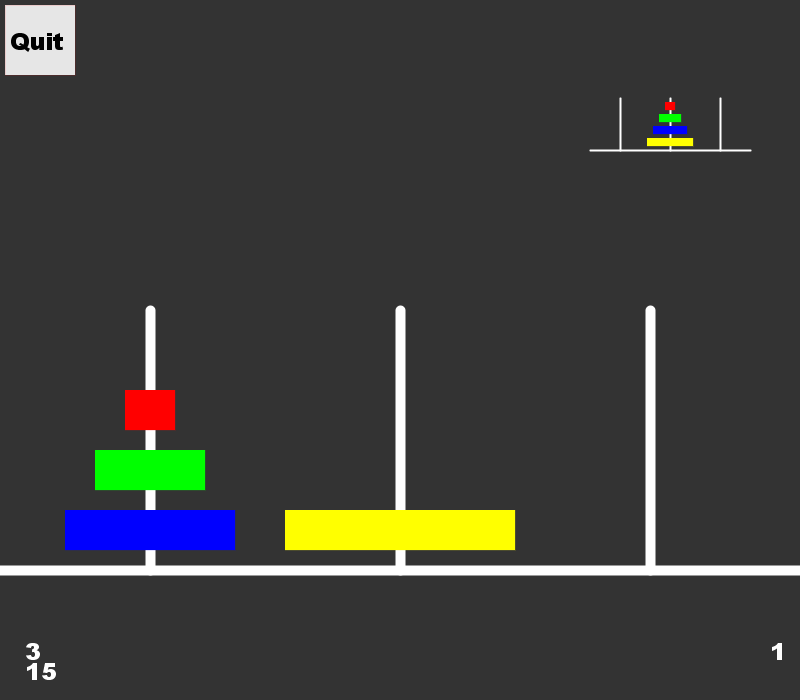
\includegraphics[height=.9\textheight]{towersofhanoi.png}}
\end{frame}

\begin{frame}{Simon's strategies}
  \begin{description}[<+->]
  \item[Goal-recursion:] To move a pyramid of size $n$ from peg $a$ to peg $b$, move a pyramid of size $n-1$ to peg $c$, ...
  \item[Perceptual] (1) Identify the largest disk that is not on the target peg; (2) Move any movable smaller disk off the source peg; (3) ...
  \item[Sophisticated Perceptual] (1) Identify the largest disk $d$ that is not on the target peg; (2) Identify the largest disk $d'$ obstructing $d$'s move; (3) Establish as a subgoal to move $d'$ to the remaining peg; ...
  \item[Move-pattern:] (1) On odd-numbered moves, move the smallest disk; (2) on even-numbered moves, move the next-smallest disk that is exposed; (3) ...
  \item[Rote learning:] Remember for every state what the optimal move is;
  \end{description}
\end{frame}

\begin{frame}{Towers of Hanoi}
  \begin{itemize}
  \item Rich mathematical tradition (state space = \alert{Sierpinski triangle}, optimal solution for 4 pegs still open);
  \item Classic algorithmic problem in computer science - shortest path algorithm recursively defined (variant of \alert{Dijkstra's algorithm} - dynamic programming);
  \item Popular task in \alert{developmental psychology} for assessing \emph{executive function} (attention, planning, etc).
    \begin{itemize}
    \item Standard analysis in psychology is checking whether for a given item, subjects have followed the optimal path
    \end{itemize}
  \end{itemize}
\end{frame}

\subsection{the Towers of Hanoi state space}

\begin{frame}{State space}
  \begin{itemize}[<+->]
  \item Every disk can be at each of the three pegs;
  \item We can represent states with for each disk (from small to large) a number indicating the peg it is on.
  \item I.e., 1133 represents a state where the smallest two disk are on the first peg, and the largest two disks on the third peg;
  \item There are $3\times3\times3\times3=81$ states.
  \item We can plot those states such that two states that can be reached from each other by a valid move are neighbours.
  \end{itemize}
\end{frame}

\begin{frame}{State space}
\scalebox{1.5}{
  \begin{picture}(150,100)
\qbezier(5,5)(27.5,45)(50,85)
\qbezier(50,85)(72.5,45)(95,5)
\qbezier(95,5)(50,5)(5,5)
\put(0,-10){1111}
\put(50,90){2222}
\put(95,15){3333}
\only<2->{\put(150,10){\vector(-2,1){100}}}
  \end{picture}
}
\only<2->{\scalebox{.5}{
  \begin{picture}(100,100)
\qbezier(5,5)(27.5,45)(50,85)
\qbezier(50,85)(72.5,45)(95,5)
\qbezier(95,5)(50,5)(5,5)
\put(0,-10){333}
\put(50,90){222}
\put(95,15){111}
  \end{picture}}}
\end{frame}

\begin{frame}%{Towers of Hanoi}
\centerline{
 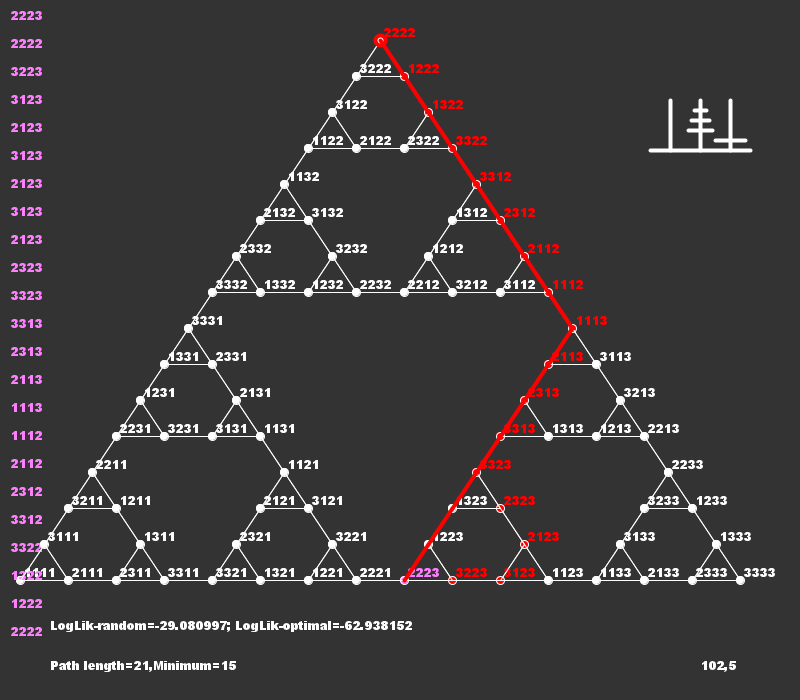
\includegraphics[height=.9\textheight]{toh.png}}
\end{frame}

\begin{frame}{Observation}
  Errors reveal much about the strategy used
\end{frame}

\section{Analysis}
\label{sec:analysis}

\begin{frame}{Shortest path}
  \begin{itemize}
  \item Standard analysis in psychology is checking whether for a given item, subjects have followed the optimal path
  \item If they do make errors, can we use the type of errors to infer something about the strategy used?
  \end{itemize}
\end{frame}

\begin{frame}{Alternative Strategies}
  \begin{description}[<+->]
  \item[Random walk:] every neighbour has identical probability of being moved to;
  \item[Optimal path (with 'performance' noise):] $p_{\mbox{optimal}}=0.9$
  \item[Subgoal-confusion:] compute sequence of subgoals on the way to the main goal, but possibly confuse subgoals with 'similar' states.
  \end{description}
\end{frame}

\begin{frame}{Subgoal-confusion: technicalities I}
  \begin{itemize}[<+->]
  \item We have a sequence of \emph{observable} moves from the subject;
  \item The subject had a sequence of subgoals in mind - but these are \emph{hidden};
  \item We thus have a number of possible subgoal-sequences we should consider;
  \item We must specify the probabilities of starting with each subgoal and transitioning to the next subgoal, as well as the probabilities of making each move given the current subgoal;
  \item Technically, this is an instance of a Hidden Markov Model, and we can compute the probability of the \emph{observed} sequence (given each possible \emph{hidden sequence and its probability}) using the Viterbi/Inside algorithm.
  \end{itemize}
\end{frame}

\begin{frame}{Subgoal-confusion: technicalities II}
I have implemented two simple subgoal-confusion models
  \begin{description}
  \item[Pyramid3confusion]: The set of candidate subgoals consists of all states with a pyramid of size 3 on the optimal path, as well as those states that have the pyramid of size 3 (but not the largest peg) on the wrong peg;
\pause
  \item[Pyramid2confusion]: The set of candidate subgoals consists of all states with a pyramid of size 2 on the optimal path, as well as those states that have the pyramid of size 2 (but not the largest peg) on the wrong peg;
  \end{description}

\pause
In both models, the player chooses a subgoal at random, and has a high probability ($p_{\mbox{remain}}=0.8$) of sticking to it. When the subgoal is reached, or with small probability otherwise, the player selects a different subgoal at random.
\end{frame}

\begin{frame}{Subgoal-confusion: behaviour}
  \begin{itemize}[<+->]
  \item These subgoal-confusion models don't model human behaviour very closely (yet);
  \item But they share with Simon's 'perceptual strategy' the property that they predict goal-directed behavior, with a high probability of moving towards a suboptimal subgoal for a while.
  \item If people are following a variant of the 'perceptual strategy' we should expect a much better fit with the data than with the predictions from the optimal strategy.
  \end{itemize}
\end{frame}

\begin{frame}{Results I: goodness of fit}
\end{frame}

\begin{frame}{Results II: consistency}
\end{frame}

\begin{frame}{Shortest paths}
\centerline{
 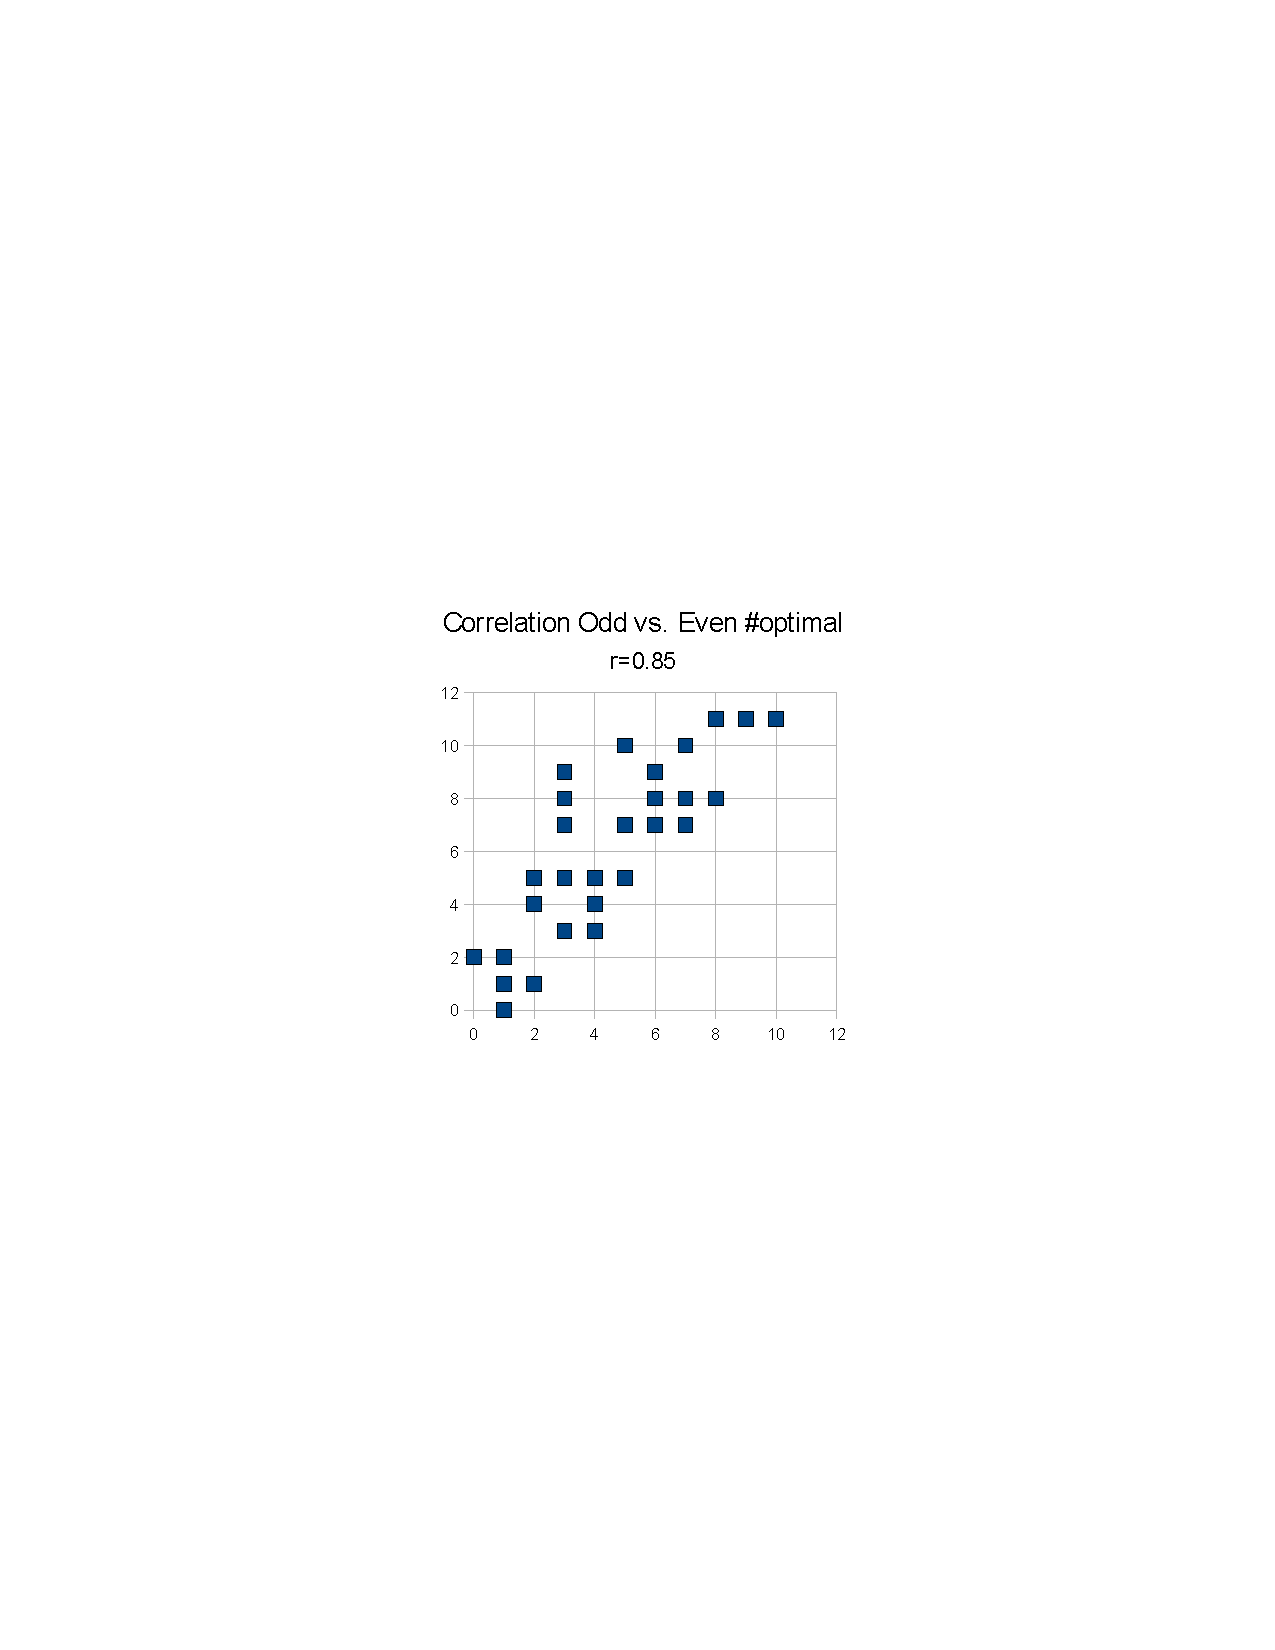
\includegraphics[trim= 10cm 10cm 10cm 10cm,height=.9\textheight]{numbershortest.pdf}}
\end{frame}

\begin{frame}{Random walk}
\centerline{
 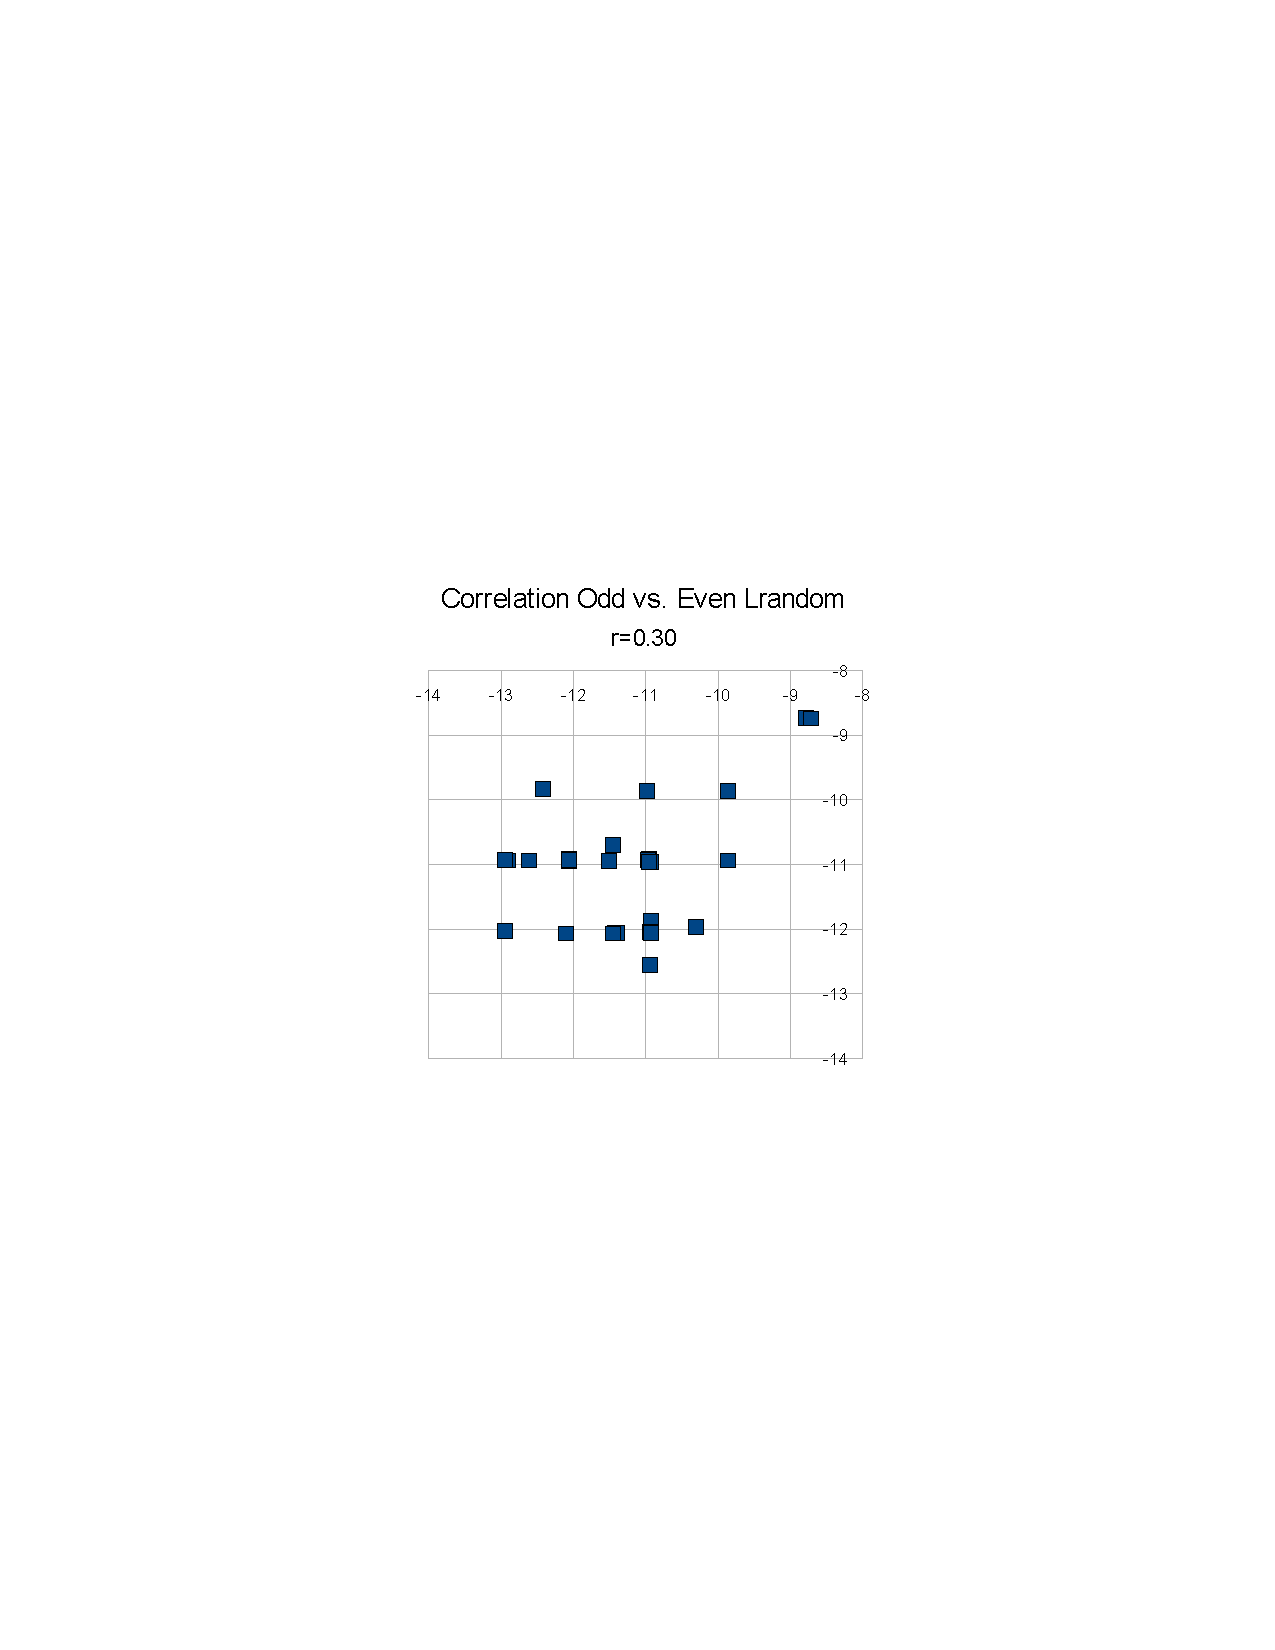
\includegraphics[trim= 10cm 10cm 10cm 10cm,height=.8\textheight]{lrandom.pdf}}
\end{frame}

\begin{frame}{Optimal path}
\centerline{
 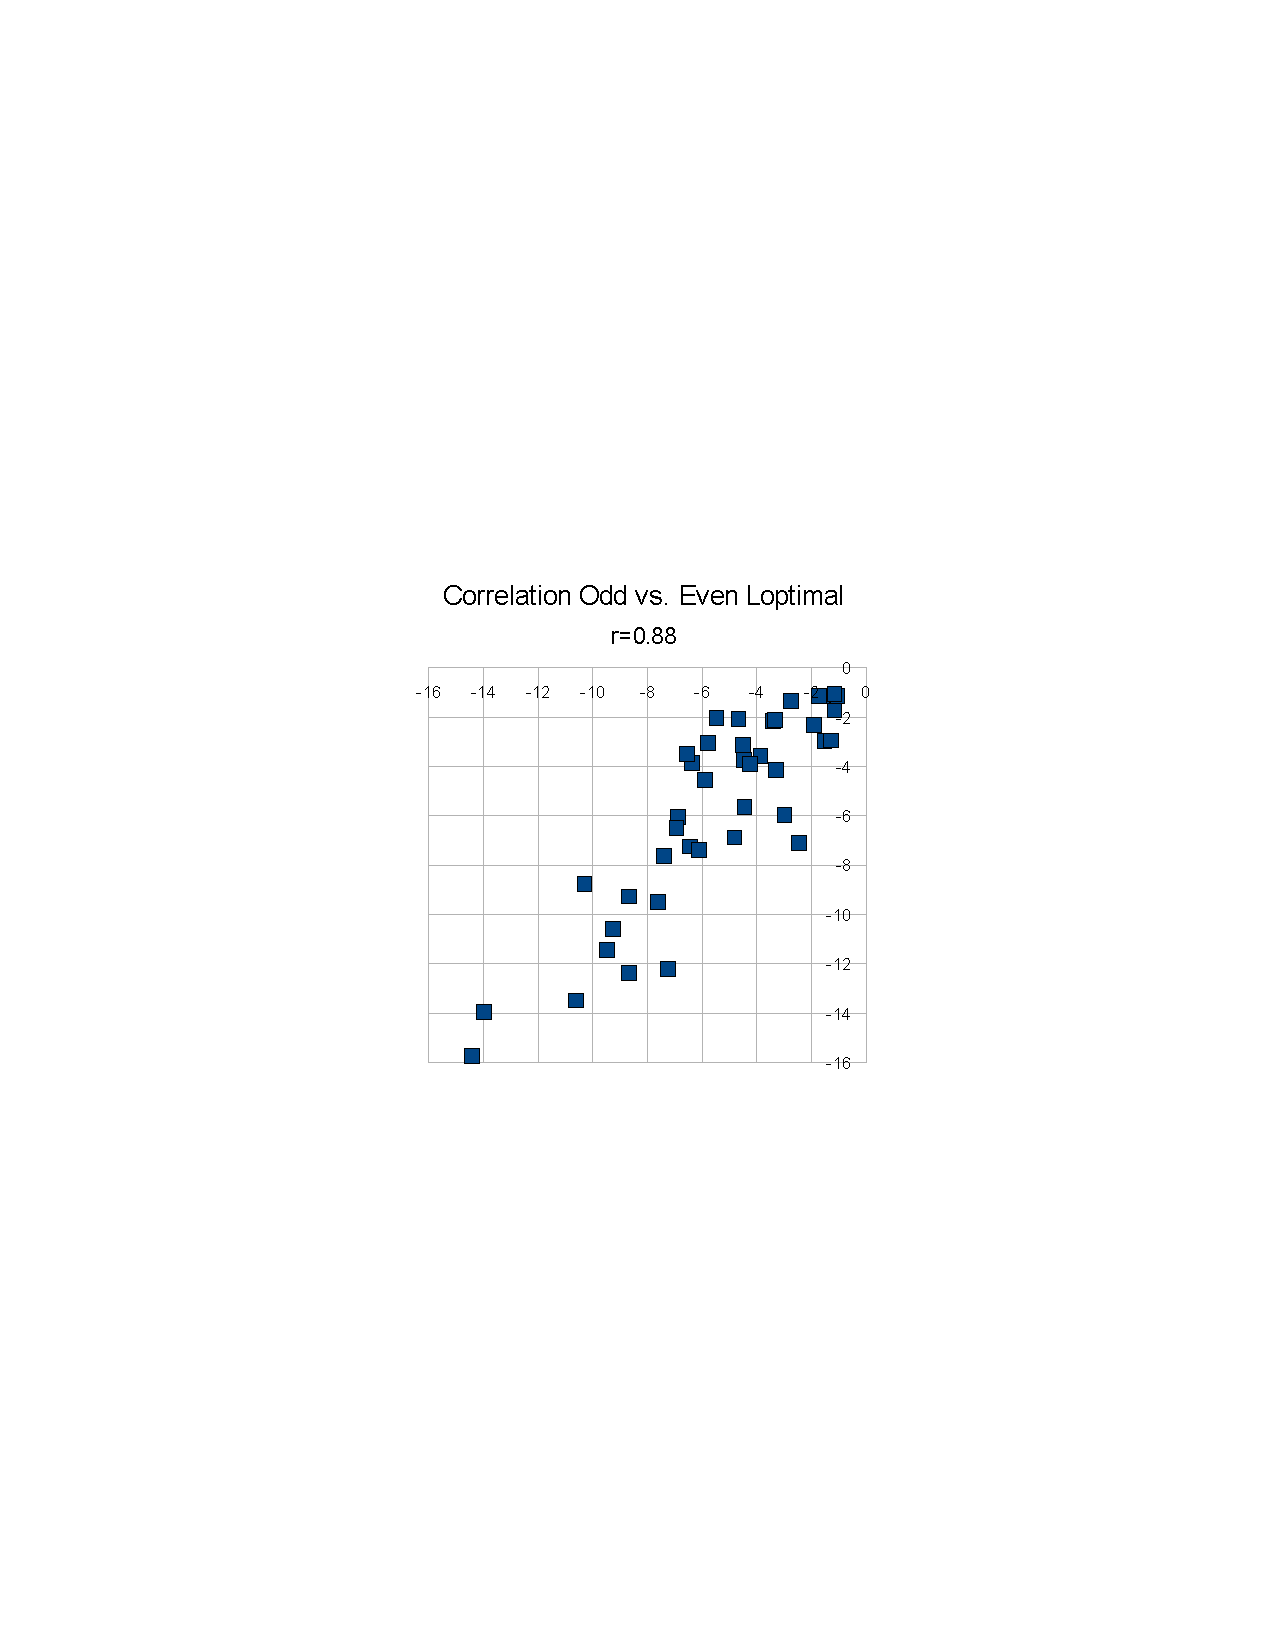
\includegraphics[trim= 10cm 10cm 10cm 10cm,height=.8\textheight]{loptimal.pdf}}
\end{frame}

\begin{frame}{Subgoal-confusion}
\centerline{
 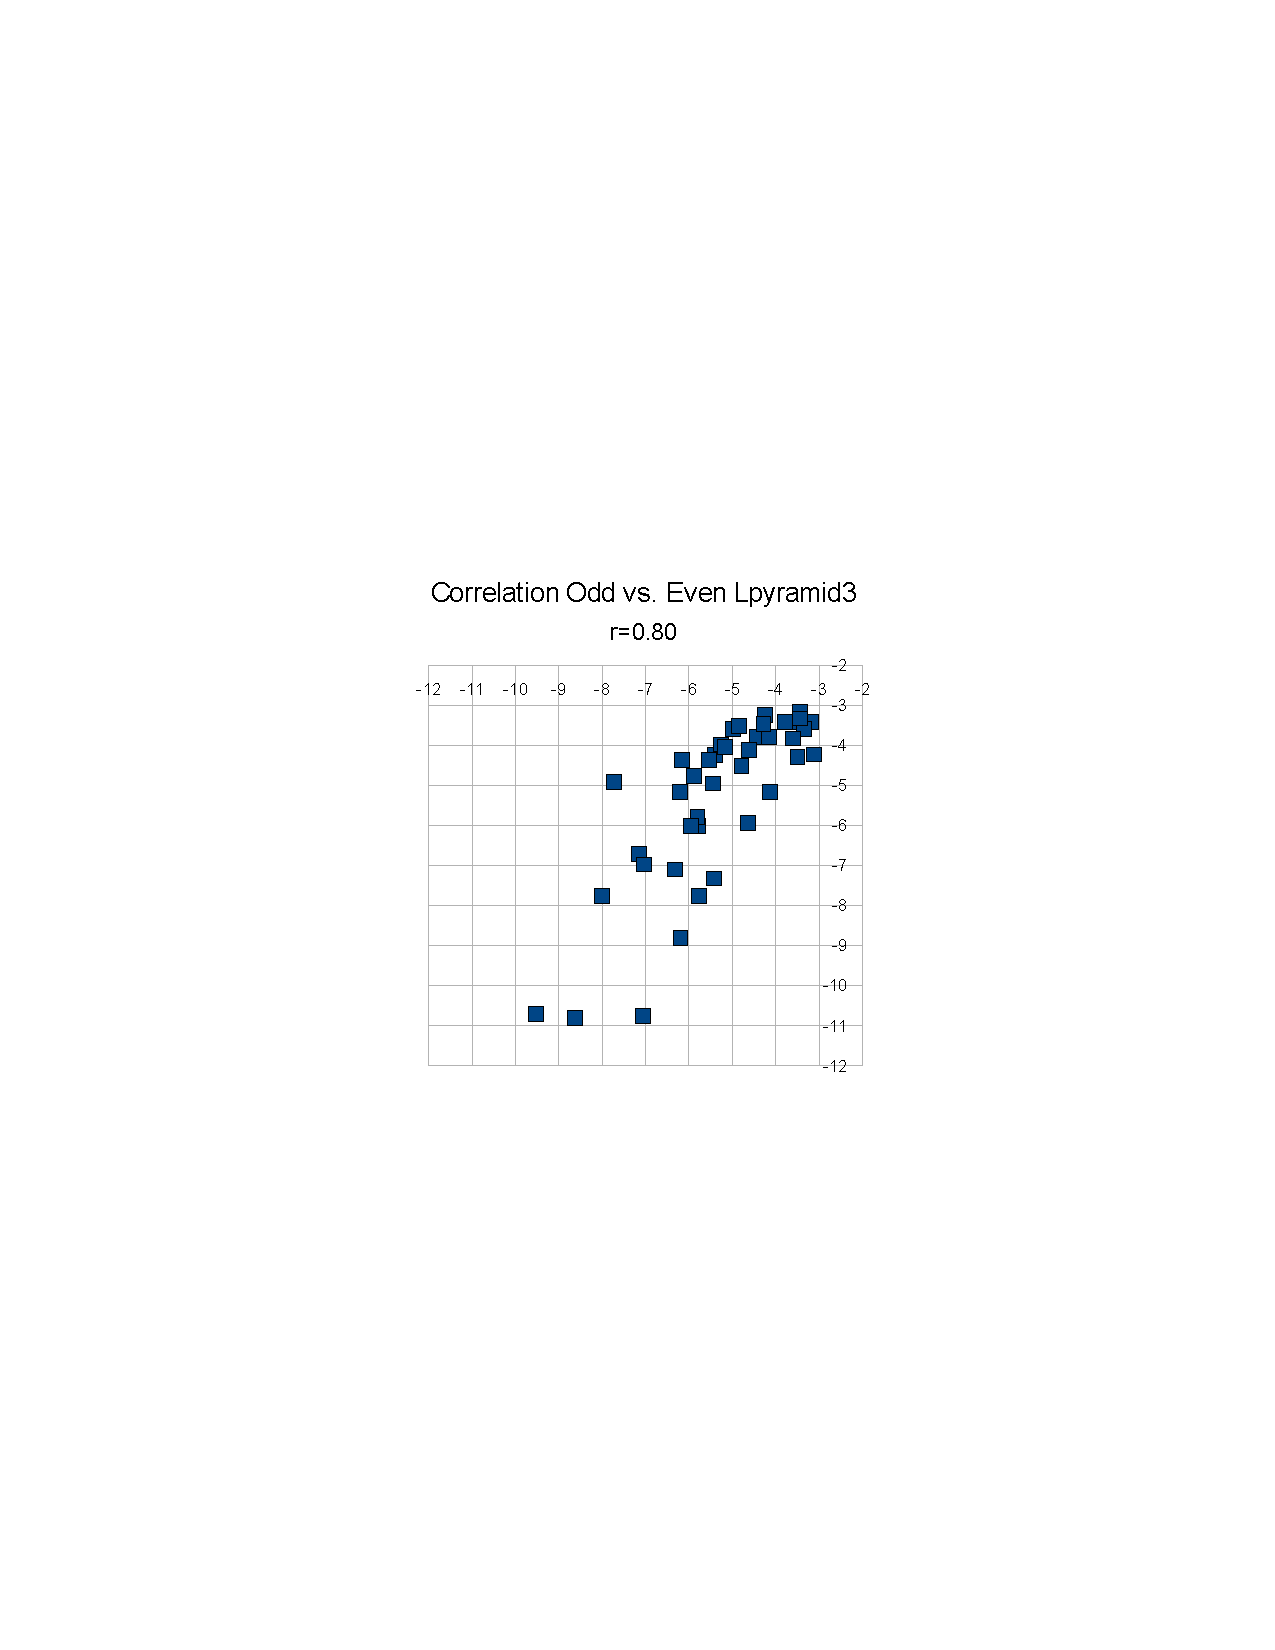
\includegraphics[trim= 10cm 10cm 10cm 10cm,height=.8\textheight]{lpyramid3.pdf}}
\end{frame}


\section{Conclusions}
\label{sec:conclusions}

\begin{frame}
  this analysis of the Tower of Hanoi problem may serve as a warning,
  illustrating the diversity of behavior that may be hidden under a
  blanket label like ``problem-solution process'' even in a very
  simple task environment. If we are to understand human
  problem-solving behavior, we must get a solid grip on the strategies
  that underlie that behavior, and we must avoid blending together in
  a statistical stew quite diverse problem solving behaviors whose
  real significance is lost in the averaging process. -- Herbert Simon
  (1975, p288)
\end{frame}


\end{document}
%---------------------------------------------------------------------------------------

